\section*{5. PHYSICAL ARCHITECTURE}

\phantomsection
\addcontentsline{toc}{section}{5. PHYSICAL ARCHITECTURE}

This chapter shows where the components of Chapter 4 run, how the nodes are connected, how data is kept, and what happens when parts of the system fail. Gate processing runs at each of the two factories, and management functions run at the central site. Each factory has its own application and database, stores its transactions locally, and sends them to the central site later. Access rights and configuration are managed centrally and sent to the factories.

\Needspace{6\baselineskip}
The deployment covers the Binh Duong and Long An factories, the TMC central site, and the existing external systems: the turnstile controllers, HR/Payroll, and TMC's email service. We use the following proposals and assumptions; TMC has to confirm them before deployment:

\begin{itemize}[leftmargin=36pt, itemsep=2pt, topsep=4pt, parsep=2pt]
  \item \textbf{Factory servers.} Each factory has a server environment for the factory application and its local database, with a standby on separate resources, so that one failure cannot stop both. Factory Monitoring runs inside the factory application. The two factories never share a database for the QR flow.
  \item \textbf{Central site.} It runs the central application, its database, the message broker, the reverse proxy, and central Monitoring.
  \item \textbf{Network.} Factories connect to the central site over a private network or VPN. APIs and messaging channels use encryption and component authentication.
  \item \textbf{Lanes.} Each lane has one kiosk and one controller. The number of lanes, server sizes, and storage capacity come from the site survey; we do not assume four lanes per factory.
  \item \textbf{Infrastructure services.} Time synchronization, backup, and key management come from the infrastructure and do not take over the responsibilities of business components.
  \item \textbf{External systems.} We assume the controller signals in I-01 and I-05 and the HR/Payroll acknowledgement in I-02. These signals, the controller protocol, and where HR/Payroll physically runs must be confirmed with their operators. Placing HR/Payroll in an integration zone in the diagram does not mean that TMC has to move it.
\end{itemize}

\Needspace{6\baselineskip}
We built the physical architecture in four steps:

\begin{itemize}[leftmargin=46pt, labelwidth=40pt, labelsep=6pt, align=left, itemsep=3pt, topsep=4pt, parsep=2pt]
  \item[\textbf{Step 1}] \textbf{Place the work.} Gate work goes to each factory and office work to the central site, following the quanta in Chapter 3 (Section 5.1).
  \item[\textbf{Step 2}] \textbf{Choose nodes and redundancy.} Each application gets the nodes it needs, with a standby only where availability requires it (Section 5.2).
  \item[\textbf{Step 3}] \textbf{Map components and connections.} Every component from Chapter 4 is placed on a node, and every link gets a protocol and a security boundary (Sections 5.2, 5.3, and 5.5).
  \item[\textbf{Step 4}] \textbf{Check quality and failures.} The 2-second budget, data persistence, and the behavior under each failure are checked against the driving characteristics (Sections 5.4, 5.6, and 5.7).
\end{itemize}


\clearpage
\subsection*{5.1. Deployment Diagram}

\phantomsection
\addcontentsline{toc}{subsection}{5.1. Deployment Diagram}

Figure 5.1 is the allocation view of TMC across the two factories, the central site, and the external systems.

\noindent\begin{minipage}{\linewidth}
\centering
\IfFileExists{diagram/deployment/figure-5-1-deployment.png}{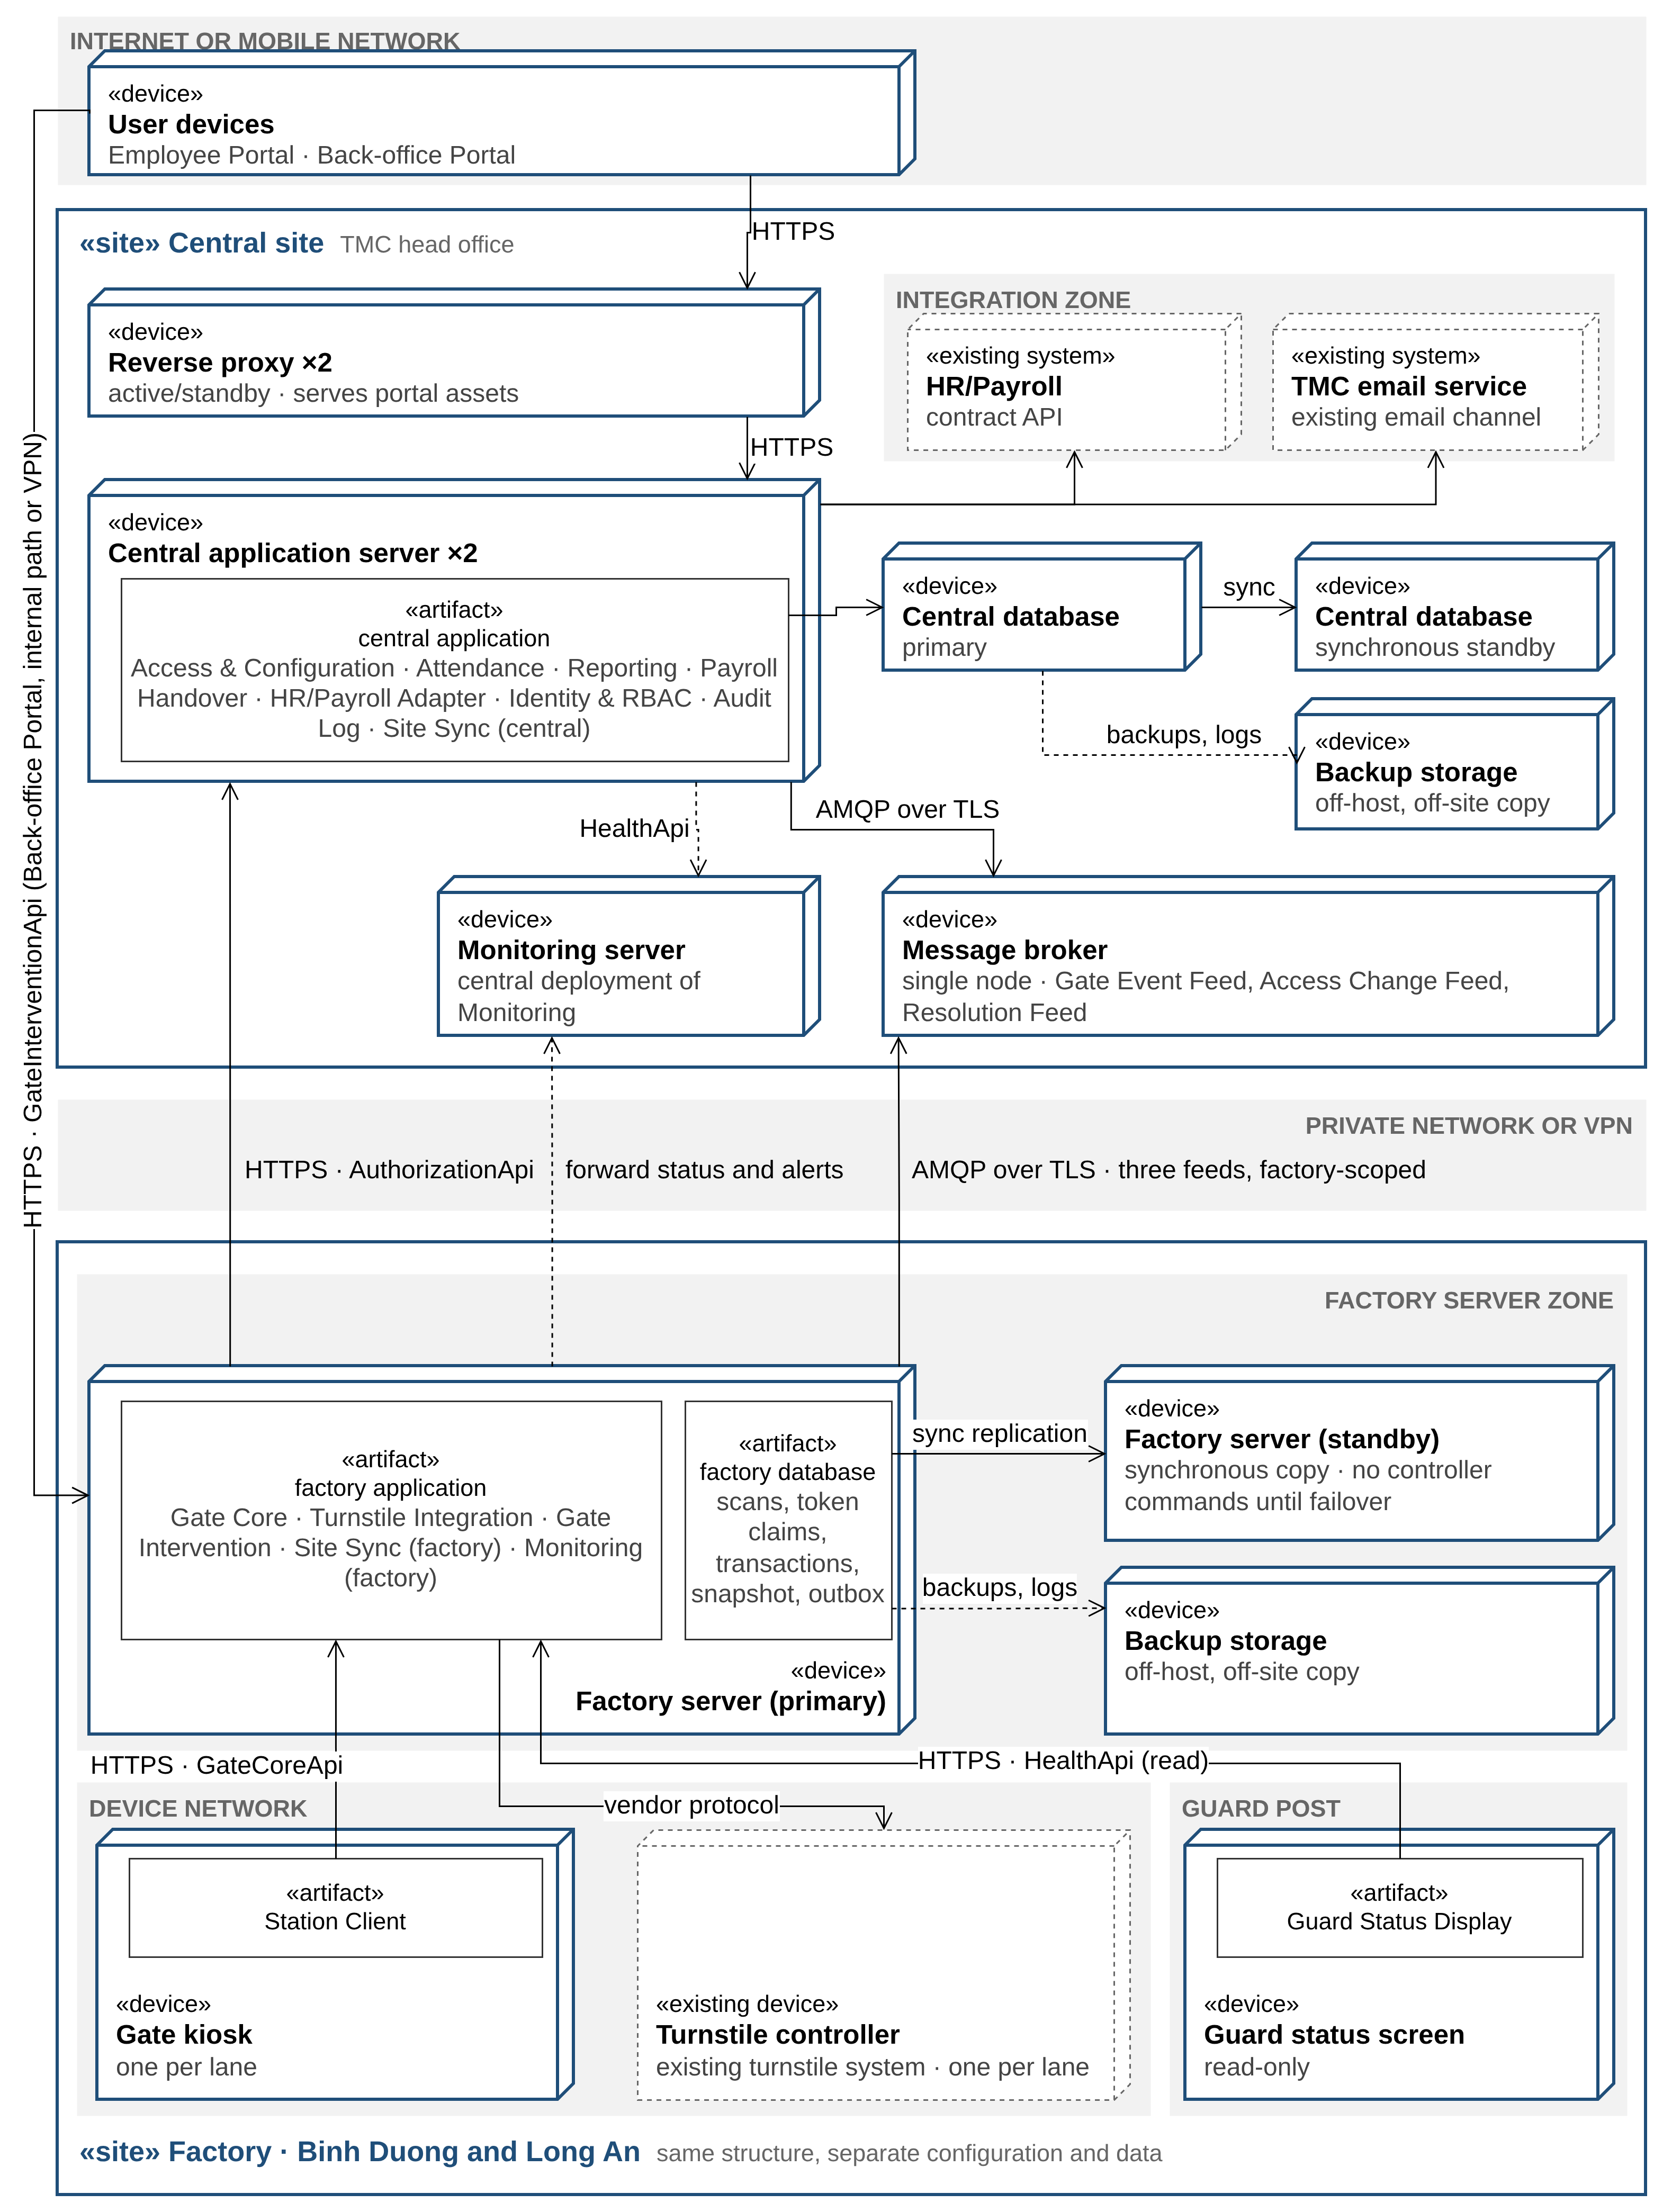
\includegraphics[width=450.0pt,height=560.0pt,keepaspectratio]{diagram/deployment/figure-5-1-deployment.png}}{\fbox{\parbox{300pt}{\centering\vspace{20pt}Figure being redrawn\vspace{20pt}}}}
\par\vspace{6pt}
\textbf{Figure 5.1. Deployment View}
\phantomsection\addcontentsline{lof}{figure}{\protect\numberline{5.1}Deployment View}
\end{minipage}

\medskip

\Needspace{6\baselineskip}
Figure 5.1 is split into three areas:

\begin{itemize}[leftmargin=36pt, itemsep=2pt, topsep=4pt, parsep=2pt]
  \item \textbf{Factory sites} (Binh Duong and Long An) share one structure with separate configuration and data. Kiosks and controllers sit in a device network that is separated from the user network. A primary and a standby factory server run the factory application and database, and the guard status screen reads factory Monitoring over the LAN.
  \item \textbf{Central site} has the reverse proxy pair, two central application instances, the central database pair, the message broker, the monitoring server, and backup storage.
  \item \textbf{External systems and user devices} are the existing turnstile controllers at each factory, HR/Payroll, TMC's email service, and the devices that run Employee Portal and Back-office Portal.
\end{itemize}

We draw the deployment in UML. Nodes labelled \guillemotleft device\guillemotright{} belong to the proposed deployment, and dashed-outline nodes are existing or external systems. Boxes labelled \guillemotleft artifact\guillemotright{} are deployed software or data, and shaded bands mark network or security zones. Solid arrows are communication paths labelled with protocols; dashed arrows are transfers of monitoring data, backups, or logs.

\Needspace{6\baselineskip}
The diagram shows two properties of the deployment:

\begin{itemize}[leftmargin=36pt, itemsep=2pt, topsep=4pt, parsep=2pt]
  \item \textbf{The QR flow stays in the factory.} Links from kiosks to the factory application and from the application to the controllers stay inside the factory network. An ordinary QR scan uses local eligibility data and waits for neither the broker nor a central call. The factory application calls central Identity \& RBAC only for assistance and intervention operations.
  \item \textbf{The factories do not depend on each other.} They never read each other's databases, so a failure at one factory does not directly stop the other. Their shared central dependencies, such as QR issuance, authorization of support operations, and access-right updates, are discussed in Section 5.7.3.
\end{itemize}

\Needspace{9\baselineskip}
\subsection*{5.2. Nodes and Component Mapping}

\phantomsection
\addcontentsline{toc}{subsection}{5.2. Nodes and Component Mapping}


Table 5.1 lists the nodes, how many of each we propose, and what they run. A node can be a physical server, a virtual machine, or another runtime environment.

\begin{longtable}{|>{\raggedright\arraybackslash}p{88pt}|>{\raggedright\arraybackslash}p{82pt}|>{\raggedright\arraybackslash}p{128pt}|>{\raggedright\arraybackslash}p{108pt}|}
\hline
\multicolumn{1}{|>{\columncolor{tableheader}\centering\arraybackslash}p{88pt}|}{\textbf{Node}} & \multicolumn{1}{>{\columncolor{tableheader}\centering\arraybackslash}p{82pt}|}{\textbf{Site and count}} & \multicolumn{1}{>{\columncolor{tableheader}\centering\arraybackslash}p{128pt}|}{\textbf{Runs or stores}} & \multicolumn{1}{>{\columncolor{tableheader}\centering\arraybackslash}p{108pt}|}{\textbf{Notes}} \\
\hline
\endhead
\multicolumn{4}{c}{\rule{0pt}{20pt}\normalsize\textbf{Table 5.1. Proposed Nodes}} \\
\endlastfoot
Gate kiosk & Each factory; one per lane & Station Client & Device network; device identity tied to factory and lane. \\
\hline
Turnstile controller & Each factory; one per lane & Existing turnstile system & Called only by Turnstile Adapter. \\
\hline
Guard status screen & Each factory; one or more at the guard post & Guard Status Display & Read-only, on the factory LAN. \\
\hline
Factory server & Each factory; one primary, one standby & Factory application (Gate Core, Turnstile Integration, Gate Intervention, factory deployments of Site Sync and Monitoring) and the factory database & Synchronous database copy; the standby sends no controller commands until failover is complete. \\
\hline
Reverse proxy & Central; one active, one standby & Entry point for users; serves portal assets & Switchover target in Table 5.5. \\
\hline
Central application server & Central; two active instances & Central application (M4--M8, M10, M11, central Site Sync) & Shared database; durable processing claims for background tasks. \\
\hline
Central database server & Central; one primary, one standby & Central database & Synchronous copy; former primary isolated on failover. \\
\hline
Message broker & Central; one node & Gate Event Feed, Access Change Feed, Resolution Feed & Durable storage; recovery target in Table 5.5. \\
\hline
Monitoring server & Central; one & Central deployment of Monitoring & Receives what the factory deployments forward. \\
\hline
Backup storage & Outside the database servers; off-site copy where possible & Database backups and archived transaction logs & Section 5.6.3. \\*
\hline\noalign{\nobreak}
User device & Anywhere & Employee Portal; Back-office Portal & No internal privileges; authorization stays on the server. \\
\hline
\end{longtable}
\phantomsection\addcontentsline{lot}{table}{\protect\numberline{5.1}Proposed Nodes}


\Needspace{6\baselineskip}
Table 5.1 lists what each node runs. The rules below explain how the nodes behave and why:

\begin{itemize}[leftmargin=36pt, itemsep=2pt, topsep=4pt, parsep=2pt]
  \item \textbf{The kiosk only scans and displays.} Station Client does not access the database, decide access rights, or call the controller; only Turnstile Adapter calls the controller API.
  \item \textbf{One active factory server.} The standby may not coordinate opening commands until a controlled failover has finished, and the former primary is isolated first, so that only one deployment writes data and drives the controller. Losing the link to the central site does not by itself trigger failover.
  \item \textbf{Guards see alerts locally.} Factory Monitoring serves the factory's status and alerts to Guard Status Display over the LAN, so guards still see alerts when the WAN link is down. Central Monitoring tracks applications, databases, devices, synchronization lag, and handover progress, and receives what each factory forwards.
  \item \textbf{Support operations need the central site.} Gate Intervention runs at the factory, but its assistance and emergency operations still need authorization from central Identity \& RBAC. A working factory application therefore does not mean that every support function works during a connectivity interruption.
  \item \textbf{Central instances share no memory state.} Neither central instance keeps critical business state only in memory, and background tasks use an exclusive processing claim, so that only one instance runs each task.
  \item \textbf{Modules keep their own data.} Modules may share a database engine, but Reporting and Payroll Handover read through the owning modules' interfaces, not from Attendance or Audit tables. Database failover must stop the former primary from accepting writes after the standby is promoted.
  \item \textbf{The broker is a single node.} It has durable storage and separate publish and consume permissions by source, factory, and message type, and recovers by restart and storage recovery. Source outboxes keep data while it is down, but they do not replace broker redundancy if TMC needs shorter interruptions.
  \item \textbf{Backups live elsewhere.} Backups are kept outside the database servers, so that one server or storage failure cannot destroy both copies.
\end{itemize}

\Needspace{13\baselineskip}
Table 5.2 shows where each component from Chapter 4 runs. Components in the same application call each other through internal interfaces, so a component does not need its own deployed service.

\begin{longtable}{|>{\raggedright\arraybackslash}p{78.5pt}|>{\raggedright\arraybackslash}p{145.5pt}|>{\raggedright\arraybackslash}p{187.5pt}|}
\hline
\multicolumn{1}{|>{\columncolor{tableheader}\centering\arraybackslash}p{78.5pt}|}{\textbf{Module}} & \multicolumn{1}{>{\columncolor{tableheader}\centering\arraybackslash}p{145.5pt}|}{\textbf{Component}} & \multicolumn{1}{>{\columncolor{tableheader}\centering\arraybackslash}p{187.5pt}|}{\textbf{Deployment location and notes}} \\
\hline
\endhead
\multicolumn{3}{c}{\rule{0pt}{20pt}\normalsize\textbf{Table 5.2. Component-to-Node Mapping}} \\
\endlastfoot
M1 Gate Core & Gate Transaction Processor; \newline Access Decision; Eligibility \newline Snapshot & Application at each factory. Each \newline deployment processes only its \newline factory's data; durable data resides \newline in the factory database. \\
\hline
M2 Turnstile \newline Integration & Turnstile Adapter & Factory application, connected to \newline the controller system within the \newline local network. \\
\hline
M3 Gate \newline Intervention & Gate Intervention & Factory application. Authorizes \newline operations through Identity \& \newline RBAC at the central site. \\
\hline
M4 Access \& \newline Configuration & Access Rights Management; \newline QR Credential Issuance; \newline Email Link Sender; \newline Gate Station Management; \newline Work Schedule Policy & Central application. Manages \newline authoritative data, sends authenticated QR-display links through TMC's existing email service, and supplies updates to factories. \\
\hline
M5 Attendance & Attendance Consolidation; \newline Attendance Review & Central application; consolidated data and review records reside in the central database. \\
\hline
M6 Reporting & Reporting & Central application; calls data-owning modules in-process and keeps no business-data copy. \\
\hline
M7 Payroll \newline Handover & Payroll Handover & Central application; batch state resides in the central database. Background work uses an exclusive processing claim. \\
\hline
M8 HR/Payroll \newline Integration & HR/Payroll Adapter & Central application, using the \newline authorized integration connection to \newline HR/Payroll. \\
\hline
M9 Site Sync & Site Sync & Deployed at each factory and at the \newline central site. These deployments \newline coordinate through the broker using \newline shared event contracts. \\
\hline
M10 Identity \newline \& Access \newline Control & Identity \& RBAC & Central application; factory support operations reach it over the protected central connection. \\
\hline
M11 Audit & Audit Log & Central application; source evidence arrives asynchronously and the central copy resides in the central database. \\
\hline
M12 \newline Monitoring \& \newline Operations & Monitoring & Central deployment for the whole system. A factory deployment inside each factory application keeps local status and alerts readable over the LAN and forwards its records to the central deployment. \\
\hline
M13 Clients & Station Client & Kiosk at each factory lane. \\
\hline
M13 Clients & Guard Status Display & Fixed screen at each factory guard post, on the factory LAN. Read-only; authenticated by a device identity checked at the factory. \\*
\hline\noalign{\nobreak}
M13 Clients & Employee Portal; \newline Back-office Portal & Interface assets are served from the \newline central site; the interfaces execute \newline on user devices. \\
\hline
\end{longtable}
\phantomsection\addcontentsline{lot}{table}{\protect\numberline{5.2}Component-to-Node Mapping}


Eligibility Snapshot only supports decisions at the factory; Access Rights Management and Gate Station Management at the central site remain the authoritative source. Site Sync and Monitoring have several deployments but one logical responsibility each. The broker only delivers messages: it does not process attendance or approve cases.

\Needspace{6\baselineskip}
\textbf{Packaging and runtime.} We propose the following packaging, to be confirmed with TMC's IT team:

\begin{itemize}[leftmargin=36pt, itemsep=2pt, topsep=4pt, parsep=2pt]
  \item \textbf{Two container images.} The factory application and the central application are each built as one container image. Both factories run the same factory image with their own configuration, so we always know which version each site runs and can return to the previous image if a release fails.
  \item \textbf{Docker on each server.} The images run under Docker on the factory servers and the central application servers. The broker, the databases, and the reverse proxy run as separate services on their own nodes (Table 5.1).
  \item \textbf{No Kubernetes.} The system has only a few nodes per site, so an orchestration platform would add operating cost without a clear benefit. It would also be risky at the factory: only one factory instance may drive the controller, and failover must isolate the former primary first, so an orchestrator must never start a second active copy on its own. If TMC already runs Kubernetes, the images can run there with one active factory instance per site.
  \item \textbf{Rolling upgrades.} Because APIs and events carry versions, the two factories and the central site do not have to be upgraded together. The central instances are upgraded one at a time, and each factory is upgraded outside its shift-change peaks.
  \item \textbf{Clients.} Station Client is installed on each kiosk and Guard Status Display on each guard screen. Employee Portal and Back-office Portal are served as static assets by the reverse proxy and run in the user's browser; authorization and business processing stay on the server. A mobile app, if TMC provides one, uses only the employee-facing contracts.
\end{itemize}

\Needspace{9\baselineskip}
\subsection*{5.3. Communication Paths}

\phantomsection
\addcontentsline{toc}{subsection}{5.3. Communication Paths}


Calls that need an immediate answer are synchronous with bounded waiting times, and data that can be processed later goes through durable messaging channels. We propose HTTPS for APIs and AMQP over TLS for the broker; controller and HR/Payroll links follow the real external APIs, and we do not assume capabilities that have not been confirmed. Table 5.3 lists the connections between nodes and external systems.

\begin{longtable}{|>{\raggedright\arraybackslash}p{95.5pt}|>{\raggedright\arraybackslash}p{147.5pt}|>{\raggedright\arraybackslash}p{168.5pt}|}
\hline
\multicolumn{1}{|>{\columncolor{tableheader}\centering\arraybackslash}p{95.5pt}|}{\textbf{From $\rightarrow$ To}} & \multicolumn{1}{>{\columncolor{tableheader}\centering\arraybackslash}p{147.5pt}|}{\textbf{Contract or purpose}} & \multicolumn{1}{>{\columncolor{tableheader}\centering\arraybackslash}p{168.5pt}|}{\textbf{Proposed communication}} \\
\hline
\endhead
\multicolumn{3}{c}{\rule{0pt}{20pt}} \\
\endfoot
\multicolumn{3}{c}{\rule{0pt}{20pt}\normalsize\textbf{Table 5.3. Connections between Nodes and External Systems}} \\
\endlastfoot
Kiosk $\rightarrow$ Factory application & GateCoreApi: submitScan, getScanStatus & HTTPS within the factory network; kiosk authentication and factory/lane scope restrictions. \\
\hline
Back-office Portal $\rightarrow$ Gate Intervention & GateInterventionApi: recordAssistedAccess, authorizeAssistedOpen, emergencyRelease, resetEmergency & HTTPS over an internal access path or VPN; server-side authorization for each operation. \\
\hline
Gate Intervention $\rightarrow$ Central Identity \& RBAC & AuthorizationApi: identity, action, and scope checks & HTTPS over a protected connection with a timeout; authorization is not bypassed on failure. \\
\hline
Factory application $\rightarrow$ Factory database & Persist states, transactions, snapshots, audit records, and outbox entries & Protected database protocol; least-privilege accounts. \\
\hline
Turnstile Adapter $\rightarrow$ Controller API & Turnstile command ports (openGate, closeGate, emergency release and reset); PASSAGE and LANE\_CLEAR are passed back to Gate Core through IPassageEvents & Vendor-supported protocol; TLS where supported, with connections restricted to the device network. \\
\hline
Factory Site Sync $\leftrightarrow$ Central broker $\leftrightarrow$ Central Site Sync & Gate Event Feed, Access Change Feed, Resolution Feed & AMQP over TLS; publishing and consumption permissions scoped by factory, source, and message type. \\
\hline
Event sources $\rightarrow$ Central Audit Log & AuditApi.append: transfer durably persisted audit evidence & Durable asynchronous channel; source validation and duplicate-safe processing. \\
\hline
User devices $\rightarrow$ Reverse proxy $\rightarrow$ Central application & Employee and management APIs & HTTPS; user authentication and server-side authorization and scope checks. \\
\hline
Central application $\rightarrow$ Central database & Read and write data according to module ownership & Protected database protocol; no direct database exposure to clients. \\
\hline
HR/Payroll Adapter $\rightarrow$ HR/Payroll API & Implementation of IPayrollSubmission & Protocol defined by the HR/Payroll contract; protection of integration credentials and handover data. \\
\hline
Central Access \& Configuration $\rightarrow$ TMC email service & Email Link Sender: deliver an authenticated link to the fresh QR display & Existing company email channel; no static QR image or reusable token in the message. \\
\hline
Data sources $\rightarrow$ Monitoring (factory or central deployment) & HealthApi: report health, errors, latency, and processing progress & Asynchronous transmission over protected connections; business flows do not wait for Monitoring to receive the data. \\
\hline
Guard Status Display $\rightarrow$ Factory Monitoring & HealthApi: read the factory's current status and active alerts & HTTPS within the factory network; device identity checked at the factory; read-only. The screen shows that its data is stale when the connection is lost. \\*
% Keep these two rows together without the break point inserted by longtable's hline.
\noalign{\nobreak}\multispan{3}\unskip\leaders\hrule height\arrayrulewidth\hfill\cr\noalign{\nobreak}
Factory Monitoring $\rightarrow$ Central Monitoring & Forward status, alerts, and measurements & Protected connection over the WAN; records are kept at the factory while the link is down. \\
\hline
\end{longtable}
\phantomsection\addcontentsline{lot}{table}{\protect\numberline{5.3}Connections between Nodes and External Systems}


Calls inside one application, such as Gate Transaction Processor to Access Decision, are internal interface calls, not network connections. Database replication and backup transfers use their own access-restricted connections, encrypted as far as the storage platform allows.

\textbf{Message delivery.} Each owning component stores the business change and its event together. Site Sync delivers persisted events through the broker, and consumers apply them by eventId and version (ADR-05). For reconciliation, Attendance Review tracks the matching ResolutionApplied after Gate Core applies the decision.

\subsection*{5.4. Response Time and Lane Capacity}

\phantomsection
\addcontentsline{toc}{subsection}{5.4. Response Time and Lane Capacity}

NFR-01 measures the time from reading the QR code to showing the opening result at the kiosk. The measured path covers validation, the ACCEPTED write, the openGate call with its OPEN\_CONFIRMED result, and the durable write of the opening result. Passage may happen later, and attendance recording, LANE\_CLEAR, and closeGate are outside the 2-second interval.

\Needspace{24\baselineskip}
Table 5.4 splits the 2 seconds over the factory-local flow. The values are targets for testing. Degraded mode uses the same local path, so the budget applies in both normal and degraded mode while the factory still accepts automatic scans.

\begin{longtable}{|>{\raggedright\arraybackslash}p{383.5pt}|>{\raggedright\arraybackslash}p{41.5pt}|}
\hline
\multicolumn{1}{|>{\columncolor{tableheader}\centering\arraybackslash}p{383.5pt}|}{\textbf{Processing stage}} & \multicolumn{1}{>{\columncolor{tableheader}\centering\arraybackslash}p{41.5pt}|}{\textbf{Budget}} \\
\hline
\endhead
\multicolumn{2}{c}{\rule{0pt}{20pt}\normalsize\textbf{Table 5.4. Proposed Response-Time Budget for a Confirmed Gate Opening}} \\
\endlastfoot
Station Client receives the QR code and prepares the request & 100 ms \\
\hline
Request transmission to the factory application and request handling & 150 ms \\
\hline
QR validation, eligibility-data lookup, and access checks & 150 ms \\
\hline
Durable persistence of the accepted scan, token claim, and traceability data & 250 ms \\
\hline
Controller invocation and receipt of OPEN\_CONFIRMED & 700 ms \\
\hline
Durable persistence of the opening result, audit evidence, and outbox event & 350 ms \\
\hline
Response transmission and display at the kiosk & 100 ms \\
\hline
\textbf{Total allocated budget} & \textbf{1,800} \textbf{ms} \\*
\hline\noalign{\nobreak}
\textbf{Reserve within the two-second limit} & \textbf{200 ms} \\
\hline
\end{longtable}
\phantomsection\addcontentsline{lot}{table}{\protect\numberline{5.4}Proposed Response-Time Budget for a Confirmed Gate Opening}


\Needspace{6\baselineskip}
The budget comes with two rules:

\begin{itemize}[leftmargin=36pt, itemsep=2pt, topsep=4pt, parsep=2pt]
  \item \textbf{Durability is never skipped.} Both durable-write steps include the standby acknowledgement required by synchronous replication. If that setup cannot meet the budget, the deployment is tuned or changed and tested again.
  \item \textbf{Deadlines.} Gate Transaction Processor checks the remaining deadline before it starts an opening command, and an expired request never starts one. If the command may already have been sent, an expired deadline does not prove that the controller did not execute it.
\end{itemize}

Table 5.4 is an allocation of the limit, not a measurement; the design must still be tested against NFR-01 at the shift-change load.

\textbf{Lane capacity.} A 2-second response does not show that the gates can carry the shift-change load, so the site survey also checks lane capacity (AC-03). For each direction, entry and exit, we estimate
\[ \mathrm{lanes} \geq \left\lceil \frac{\mathrm{peak\ rate} \times \mathrm{gate\ cycle\ time}}{\mathrm{target\ utilization}} \right\rceil \]
The peak rate is about 1.33 events per second per factory (400 events in 5 minutes), but it counts entries and exits together, so the survey must split it by direction. The gate cycle time runs from ACCEPTED until the lane is released and must be measured on the real turnstiles; it is not the 15-second passage-observation limit. TMC sets the target utilization to leave room for queues and rescans. We do not fix the number of lanes until these values are measured.

\Needspace{9\baselineskip}
\subsection*{5.5. Security Boundaries}

\phantomsection
\addcontentsline{toc}{subsection}{5.5. Security Boundaries}


The deployment uses the following network and security boundaries:

\begin{itemize}[leftmargin=36pt, itemsep=2pt, topsep=4pt, parsep=2pt]
  \item \textbf{Factory zones.} The factory network is split into kiosk, application, and controller-device zones, and firewalls allow only the connections that are needed between them.
  \item \textbf{Kiosk identity.} Each kiosk has a device identity tied to its factory and lane, for example a device certificate. The server checks each request against the registered configuration instead of trusting the factory or lane values in the request. A kiosk may only submit scans and query their status; it cannot call recordIntervention, change configuration or access rights, or trigger emergency opening.
  \item \textbf{Controller access.} Only Turnstile Adapter connects to the controllers; users, kiosks, and the central application have no path that bypasses the factory application. If a controller does not support TLS, we record this limitation and rely on isolation in the device network and restricted sources; we do not call that link end-to-end TLS.
  \item \textbf{Central entry point.} The reverse proxy is the entry point for user access. The central application, database, and broker are not exposed to external networks, and factories reach only the endpoints and channels they need.
  \item \textbf{Factory scope.} Site Sync at a factory may publish events and receive updates only within that factory's scope. Factories cannot publish authoritative access-right changes or approval decisions on behalf of Attendance Review.
  \item \textbf{Integration credentials.} HR/Payroll Adapter uses a dedicated integration account limited to the handover contract. Kiosks and factory applications never access the payroll database or use the adapter's credentials.
  \item \textbf{Verification keys.} Factories receive only the material they need to verify QR codes, and holding it does not let a factory issue tokens. Key management and replay prevention are described in Chapter 7.
  \item \textbf{User access and personal data.} The reverse proxy and application services check operation and data-scope permissions before any request reaches central data. Database, broker, and backup access is limited to the matching service and administrator accounts. Chapter 7 covers audit access and personal-data protection for these records.
\end{itemize}

\Needspace{9\baselineskip}
\subsection*{5.6. Data Persistence and Availability}

\phantomsection
\addcontentsline{toc}{subsection}{5.6. Data Persistence and Availability}

\subsubsection*{5.6.1. Persistence}

\phantomsection
\addcontentsline{toc}{subsubsection}{5.6.1. Persistence}


Each site keeps its own records durably:

\begin{itemize}[leftmargin=36pt, itemsep=2pt, topsep=4pt, parsep=2pt]
  \item \textbf{Factory database.} It holds scan and gate-cycle states, token claims, passage evidence, source attendance transactions, audit evidence, support cases, the eligibility data used for decisions, duplicate-prevention data, and pending events. Gate Transaction Processor stores ACCEPTED and the token claim together before a controller command, and a confirmed passage is stored with its attendance transaction and outgoing event. Controller actions are outside the database transaction, so recovery may need controller evidence or reconciliation.
  \item \textbf{Central database.} It holds authoritative access rights and configuration, shift schedules, consolidated attendance, review cases, decisions and evidence, audit copies, HR/Payroll batch content and receipt history, and accounts and permissions. Attendance Review tracks application at Attendance Consolidation and Gate Core separately. Payroll Handover stores batch identity and content before external submission, and competing central instances use durable processing claims.
\end{itemize}

\subsubsection*{5.6.2. Redundancy and Failover}

\phantomsection
\addcontentsline{toc}{subsubsection}{5.6.2. Redundancy and Failover}

The primary database acknowledges a commit only after the data is stored as the synchronous replication setting requires. Acknowledged commits therefore survive a primary failure while the standby is intact. The price is that the standby becomes part of every write: if the commit conditions cannot be met, the system does not silently switch to weaker persistence while still reporting success.


At a factory, this rule has a direct consequence. If the primary database cannot get the required standby acknowledgement, for example because the standby or the replication link has failed, the factory stops accepting new scans that would lead to an opening command. Cycles that are already open must still end safely. Gate Core continues automatic closing only while it can still durably record LANE\_CLEAR and the single reserved close command; otherwise guards close or secure the lane under the approved safety procedure. Passage or attendance that could not be stored is reconciled from controller evidence after recovery, and in-progress scans are resolved the same way. Guards use the manual procedure for new arrivals, and attendance recording is never moved to the kiosk to get around the database failure. The remedy is to repair the standby or the replication link, not to fail over, because the primary is still working. We keep this policy because ADR-10 does not allow durability to be weakened during a failure.


Failover covers the other case: the primary fails and an eligible standby can take over. After promotion, the new primary has no synchronous partner, so under the same rule it still cannot accept new scans until a replica can acknowledge commits again. Changing roles is therefore not the end of recovery. The 5-minute target in Table 5.5 is measured until the commit conditions are restored and new scans are accepted. Meeting it may need a second standby or a replica that can be rebuilt quickly; testing decides which.


At the central site, the reverse proxy stops routing requests to an unavailable application instance, and the other instance carries on from database state. Database failover must isolate the former primary before the promoted database accepts writes.


Replication does not protect against every failure. Accidental deletion, wrong updates, or corrupted data are copied to the standby as well, and losing both copies or a whole site still needs a backup restore.

\subsubsection*{5.6.3. Backup and Restore}

\phantomsection
\addcontentsline{toc}{subsubsection}{5.6.3. Backup and Restore}

We propose a daily full database backup and continuous transaction-log archiving, with log transfer normally no more than five minutes behind. Backups are stored outside the database servers, with an off-site copy where the infrastructure allows. They cover scan states, token claims, transactions, decisions, audit records, batches, outboxes, and deduplication markers. Configuration, active contracts, and the information needed for key recovery need their own retention.


After a restore, the application does not accept new scans until database state, application versions, unfinished scans, eligibility data, and replay-prevention state have been checked. A restore may take the data back to an earlier point in time, so tokens used and commands executed after that point must be handled under a safe recovery policy. They are never treated as if they had not been processed.


\Needspace{6\baselineskip}
Data-loss and recovery objectives depend on the failure scope:


\begin{itemize}[leftmargin=36pt, itemsep=2pt, topsep=4pt, parsep=2pt]

  \item For an isolated primary-database failure with an intact synchronous standby, the objective is to lose no acknowledged commits.

  \item For failures that need a backup restore, the initial objective is a data-loss window of no more than five minutes, provided log archiving works correctly.

  \item Site-wide loss, simultaneous failures, and incomplete log transfer are assessed separately.

\end{itemize}

The five-minute window applies only to failures; it does not relax NFR-02's requirement to keep attendance records during normal operation. Any part that cannot be recovered exactly is recorded and reconciled.

\subsection*{5.7. Failure Handling and Recovery}

\phantomsection
\addcontentsline{toc}{subsection}{5.7. Failure Handling and Recovery}

Failures are handled with explicit thresholds, a bounded degraded mode at the factories, and a fixed recovery order after reconnection.

\Needspace{9\baselineskip}
\subsubsection*{5.7.1. Operating Thresholds}

\phantomsection
\addcontentsline{toc}{subsubsection}{5.7.1. Operating Thresholds}


Table 5.5 sets initial thresholds for configuration and testing. TMC must approve the two access-right limits (60 seconds and 30 minutes) because they decide how quickly a revocation takes effect.

\begin{longtable}{|>{\raggedright\arraybackslash}p{95.5pt}|>{\raggedright\arraybackslash}p{156.5pt}|>{\raggedright\arraybackslash}p{158.5pt}|}
\hline
\multicolumn{1}{|>{\columncolor{tableheader}\centering\arraybackslash}p{95.5pt}|}{\textbf{Item}} & \multicolumn{1}{>{\columncolor{tableheader}\centering\arraybackslash}p{156.5pt}|}{\textbf{Threshold or objective}} & \multicolumn{1}{>{\columncolor{tableheader}\centering\arraybackslash}p{158.5pt}|}{\textbf{Application}} \\
\hline
\endhead
\multicolumn{3}{c}{\rule{0pt}{20pt}\normalsize\phantomsection\addcontentsline{lot}{table}{\protect\numberline{5.5}Proposed Operating Thresholds and Recovery Objectives}\textbf{Table 5.5. Proposed Operating Thresholds and Recovery Objectives}} \\
\endlastfoot
Kiosk response while automatic scans are accepted & No more than 2 seconds, in normal and degraded mode & The NFR-01 limit, not a configurable threshold for relaxing the requirement. \\
\hline
Controller interaction during a QR scan & Initial budget of 700 ms, without exceeding the scan's remaining deadline & Applies only to openGate in the QR flow. If the deadline has already passed, no command is sent. Expiration after the command may have been sent is treated as an undetermined outcome. \\
\hline
Controller interaction during an assisted opening & Initial time limit of 3 seconds, configurable & A threshold we chose for the guard-assisted flow, separate from the kiosk response target in NFR-01. A timeout after the command may have been sent is undetermined, and the command is never resent. \\
\hline
QR token validity (I-09) & 60 seconds from issuance & Reject the expired token for its scan; other valid tokens may still be accepted. \\
\hline
Passage observation (I-05) & Initial 15 seconds after OPEN\_CONFIRMED & Gate Core flags missing passage for review. This timer never authorizes closeGate. \\
\hline
Component health checks & Every 5 seconds; alert after 3 consecutive failures & Approximately 15-second detection target, to be measured in testing. Failures encountered by actual requests are handled immediately. \\
\hline
Access-right update progress confirmation & Proposed interval of 10 seconds & Confirmation must identify versions and applied progress, not merely indicate that the connection is alive. \\
\hline
Normal age of access-right data (I-10) & No more than 60 seconds from the source's confirmation of a valid data watermark, allowing for transmission delay and clock skew & Normal automatic acceptance. Past this limit the factory switches to degraded mode if the other conditions in Section 5.7.2 still hold. \\
\hline
Degraded-mode limit (I-10) & Less than 30 minutes from the same watermark & Accept only signed, unexpired, unclaimed QR codes and flag each transaction. Once the data is 30 minutes old, or continuity is lost, stop automatic acceptance at all lanes; new scans return CANNOT PROCESS. \\
\hline
Clock error used for validity checks & Below 2 seconds against the time used for QR issuance and checkpoints & Continue only while the factory has a measured error bound below the limit. Stop QR processing when the bound is lost or reaches or exceeds the limit (Section 5.7.2). \\
\hline
Outbox storage capacity & Sized for at least 48 hours under the load model; warning at 70\% utilization and critical alert at 85\% & Do not delete events that have not met delivery conditions merely to free storage. \\
\hline
Failover after a primary failure & No more than 5 minutes from the start of the procedure until commit conditions are restored and new scans are accepted & Only when the primary has failed and an eligible standby can take over; the former primary is isolated first. A failed standby is repaired, not used for failover (Section 5.6.2). \\
\hline
Recovery of the broker and Access Change Feed & Proposed: no more than 10 minutes, to be verified. Measured from detecting the broker outage until each factory has applied the backlog and advanced its watermark with a new confirmed checkpoint & Leaves a margin before the 30-minute limit in I-10. A longer outage stops automatic scans at the factories one after another (Section 5.7.3). \\
\hline
Switchover of the reverse proxy & Proposed: no more than 30 seconds, to be verified. Measured from detecting the proxy failure until a new QR code is issued successfully through the standby proxy & Shortens the interruption to new QR issuance. Codes already shown keep their own 60-second validity and may still expire during the switchover. \\
\hline
Database restoration from backup & Initial target of no more than 30 minutes with the test dataset & Measure until data and service-readiness conditions have been checked; this is not a guarantee for every data volume or failure. \\
\hline
Synchronization after connectivity is restored & Sustained processing rate of at least twice the event-generation rate in the test & Receive new data while reducing the backlog; verify using a representative load model. \\*
\hline\noalign{\nobreak}
HR/Payroll handover & First submission planned at 06:00; internal alert at 10:00; required data available before 12:00 noon on day one & Check overnight shifts and source progress; 06:00 is not a final cutoff. Alerts do not replace confirmation. \\
\hline
\end{longtable}


Outbox capacity is sized from real event counts and sizes, audit data, retransmissions, and a reserve; the load of 800 events in 30 minutes does not last all day. When storage reaches the critical threshold, operators estimate how long data can still be kept. The application stops accepting new scans before space runs short for mandatory transactions and the recovery reserve, not when the database is already full.

\subsubsection*{5.7.2. Eligibility Freshness and Degraded Mode}

\phantomsection
\addcontentsline{toc}{subsubsection}{5.7.2. Eligibility Freshness and Degraded Mode}

Eligibility Snapshot is used only when its data is complete, comes from an authorized source, and meets the version, continuity, and time requirements.


The Access Change Feed keeps sending progress confirmations even when nothing changes, so that a factory can tell how far it has received. Each confirmation carries the time at which the source checked and confirmed the data watermark. The factory advances its watermark only after applying all required data up to that point. Freshness is measured from the source's time, allowing for transmission delay and clock error, so a delayed message does not restart the 60-second limit. Duplicates, older versions, health signals without progress information, and the update time of a single record cannot refresh the watermark.


\Needspace{6\baselineskip}
The QR flow continues only when all of the following conditions hold:


\begin{itemize}[leftmargin=36pt, itemsep=2pt, topsep=4pt, parsep=2pt]

  \item The QR token is valid and unexpired.

  \item Employee data, access rights, lane configuration, and verification keys have the required versions.

  \item No missing sequence or unapplied mandatory update has been detected.

  \item The watermark is within the normal limit, or within the degraded limit described below.

  \item The clock-error bound is known and below 2 seconds.

  \item The factory application, database, and controller are working.

  \item Token claiming and replay prevention work as described in Chapter 7.

  \item Enough storage capacity remains.

\end{itemize}

Losing the connection does not invalidate a token or the snapshot at once, but their limits in Table 5.5 keep running, and an expired token is rejected for its own scan. When the watermark passes 60 seconds, Gate Core switches the factory to degraded mode instead of stopping. Because the watermark may already be a few seconds old when the link fails, this can happen in less than one minute.


\Needspace{6\baselineskip}
\textbf{Degraded mode.} Gate Core keeps the normal flow with three changes:

\begin{itemize}[leftmargin=36pt, itemsep=2pt, topsep=4pt, parsep=2pt]

  \item It accepts only QR codes whose signature is valid under the locally stored key, that are unexpired, bound to this factory, and not yet claimed. Replay protection does not change, because all lanes share the factory's token-claim data.

  \item It marks every ACCEPTED scan, and the attendance transaction created after passage, with a DEGRADED flag and the snapshot version it used.

  \item It writes the start and end of the mode to the audit log and raises an alert through the factory deployment of Monitoring. Guard Status Display shows the alert at the guard post over the factory LAN, and the central deployment receives it when the link returns. The kiosk shows the employee the normal result.

\end{itemize}

The mode ends in one of two ways. If confirmed updates arrive again, Site Sync applies the missing changes and Gate Core returns to normal mode. Attendance Review then compares each DEGRADED transaction with the changes that were applied. A transaction whose employee was suspended, lost access, or was moved to another factory during the window becomes a review case for HR or Security; the others stay flagged in reports. If 30 minutes pass since the last confirmed update, Gate Core returns CANNOT PROCESS for new scans at every lane and guards use the approved manual procedure. In both cases an opened lane still needs passage tracking and safe closing.


We chose 30 minutes because it covers one full shift-change peak (about 800 scans per factory). Every scan in the window is flagged, but only transactions whose employee's access changed during the window become review cases, so HR does not have to check all of them. The value is a configuration parameter, and TMC must approve it together with the revocation risk below.


\textbf{Factory WAN outage and central outage.} New QR codes still come from the central site, but an employee's phone reaches it over the Internet or the mobile network, not over the factory WAN link. During a factory WAN outage, employees can therefore still get fresh codes and pass in degraded mode. A central-site outage is different: QR issuing stops, existing codes expire within 60 seconds, and the automatic flow stops at both factories at about the same time, whatever the state of the snapshot.


Guards switch to the approved manual procedure only when automatic acceptance is no longer allowed. During a central-site outage this happens once existing codes expire. During a factory WAN outage it happens when the watermark reaches the I-10 limit, or earlier if the factory no longer meets another required operating condition, such as a known clock-error bound, durable writes, or snapshot continuity. Each manual entry is recorded as an assisted case that HR must approve (I-04). During a central-site outage, software authorization for assisted opening is also unavailable (Section 5.7.4), so guards keep the record by hand and enter it after recovery. Arrivals average about 27 per minute per factory over the 30-minute shift change, and we assume a peak of about 80 per minute (400 events in 5 minutes). TMC needs a staffing plan for that peak. The software never lets a kiosk open the gate on its own.


Each token is valid at only one factory, and all lanes in that factory share Gate Core's token-claim data. Acceptance during a disconnection is allowed only while replay prevention works and all eligibility-data conditions hold. If token-claim consistency cannot be guaranteed after failover or restoration, the factory stops accepting new scans until safe conditions are re-established.


\textbf{Time during a WAN outage.} The factory application server is the time source for the kiosks and synchronizes with the time used for QR issuance and checkpoints at the central site. What matters is the error against that central time; factory clocks that agree with each other can still all be wrong. Gate Core keeps an error bound: the error measured at the last successful synchronization plus the drift allowed since then, using a drift rate measured for the server in testing. The bound grows while the WAN is down. Gate Core continues QR checks only while the bound is known and below 2 seconds, and stops automatic acceptance when it cannot establish the bound or the bound reaches or exceeds the limit (Table 5.5). The central issuing service follows the same rule for its own clock.


\textbf{Effectiveness of access-right revocation.} Once a factory receives and applies a change, new scans use the updated version. During isolation, the factory may not know that a right has just been revoked at the central site. Automatic acceptance using the old rights is allowed only while the last confirmed watermark is less than 30 minutes old. The revocation itself may arrive later, after reconnection; 30 minutes is not a delivery guarantee. The DEGRADED flag makes every scan in that window easy to find and check later, but it cannot undo an entry that has already happened. If TMC needs immediate revocation, the scans that need that guarantee must check online or stop when the connection is down. The system cannot rely on a disconnected copy and also know every central change at once.

\subsubsection*{5.7.3. Loss of Central Connectivity or Broker Availability}

\phantomsection
\addcontentsline{toc}{subsubsection}{5.7.3. Loss of Central Connectivity or Broker Availability}

When the central site or the broker cannot be reached, the factory keeps new passage-based attendance transactions and other events in its local outbox, and accepts new scans only under the conditions in Section 5.7.2. Passage tracking and closeGate stay local and do not wait for the broker. Operations that need central authorization, such as software-based assistance and emergency opening, may stop. Whether employees can still get new QR codes depends on whether their phones can reach the central application, not on Site Sync.


If only the broker is unavailable, central APIs may continue operating while the central application and database remain available. Gate-transaction delivery, access-right updates, and reconciliation decisions are delayed, and reports may lack recent factory data. Because the Access Change Feed also stops, neither factory receives new checkpoints. Each factory moves to degraded mode when its watermark passes 60 seconds and stops automatic acceptance when it reaches 30 minutes. The factories cross these limits one after another, since their last checkpoints differ. For this reason the recovery target in Table 5.5 covers the whole path, not only restarting the broker.


\textbf{Shared central entry points.} The broker and the reverse proxy are both shared by the two factories, but losing them has different effects. Losing the reverse proxy blocks the route to QR issuance, so automatic scans fail at both factories within about 60 seconds as existing codes expire. Losing the broker only ages the watermark, which leaves up to 30 minutes. We therefore run the reverse proxy as an active/standby pair and keep the broker as a single node with the recovery target in Table 5.5. Two central application instances do not cover either failure.


\textbf{After reconnection.} Site Sync checks versions, applied watermarks, and pending data. Missing access-right updates are fetched as a change sequence or as a complete snapshot from an authorized source, and Access Decision uses them only after the required conditions are checked again, not just because the link is back. Transaction and audit events are resent with their original identifiers. The central site processes backlog and new data together, with resource limits so that catching up does not slow the QR flow. Reports show reception progress and missing data; the timestamp of the newest event does not prove that all earlier events have arrived.

\noindent\begin{minipage}{\linewidth}
\setlength{\parskip}{0pt}
\setstretch{1}
Figure 5.2 shows the recovery order after the link to the central site returns.
\par\vspace{8pt}
\centering
\IfFileExists{diagram/deployment/figure-5-2-reconnect.png}{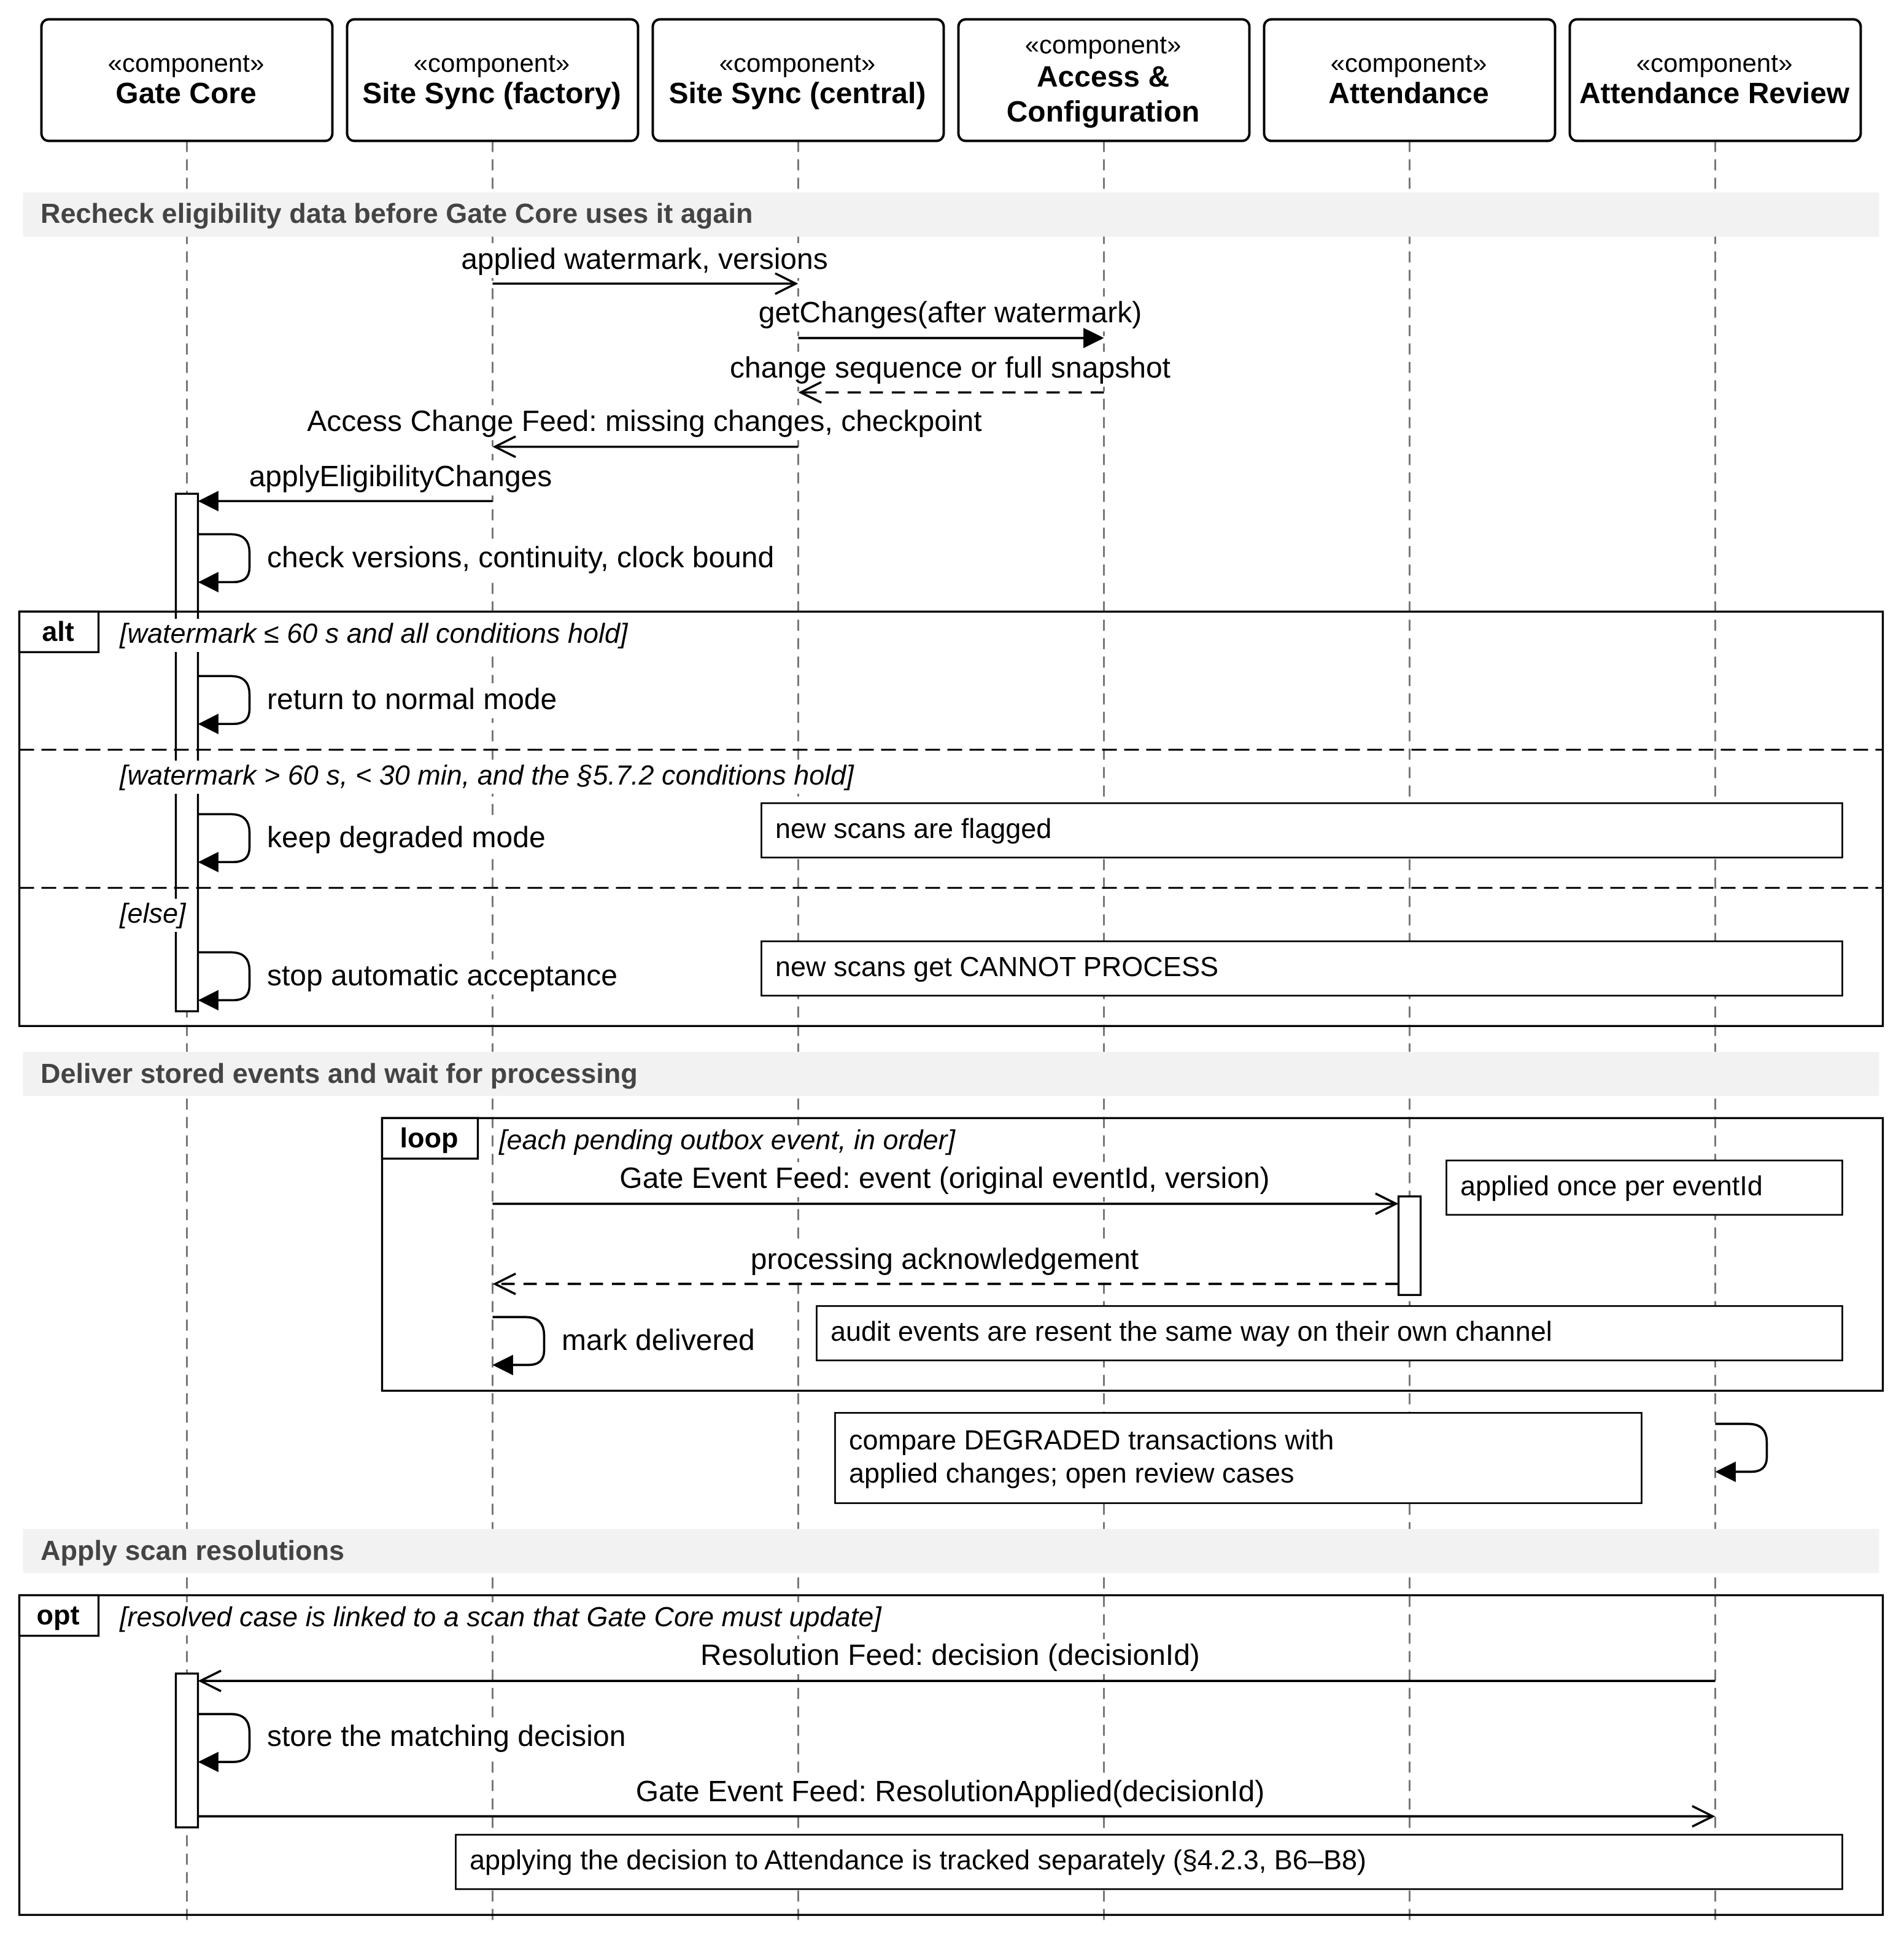
\includegraphics[width=450.0pt]{diagram/deployment/figure-5-2-reconnect.png}}{\fbox{\parbox{300pt}{\centering\vspace{20pt}Figure being redrawn\vspace{20pt}}}}
\par\vspace{4pt}
\textbf{Figure 5.2. Recovery Order after Reconnection}\par
\phantomsection\addcontentsline{lof}{figure}{\protect\numberline{5.2}Recovery Order after Reconnection}
\vspace{6pt}
{\raggedright
In this order, Site Sync rechecks source versions and applied watermarks before Gate Core uses eligibility data again, then sends stored events with their original identifiers and waits for each consumer's processing acknowledgement. When a resolved case is linked to a scan that Gate Core must update, it follows steps B6--B8 of Flow B and is complete only after Gate Core stores the matching decision and returns ResolutionApplied. Applying the decision to Attendance is tracked separately. The Access Change Feed, Gate Event Feed, and Resolution Feed shown here pass through the message broker. No recovery step resends openGate.
\par}
\end{minipage}

\medskip

\Needspace{12\baselineskip}
\subsubsection*{5.7.4. Other Failures}

\phantomsection
\addcontentsline{toc}{subsubsection}{5.7.4. Other Failures}


Three other failure areas need their own handling:

\begin{itemize}[leftmargin=36pt, itemsep=2pt, topsep=4pt, parsep=2pt]
  \item \textbf{Factory application, database, and controller.} A kiosk that loses its response keeps the scanId and queries the stored result after reconnection. During factory-application failover, new scans stop while Gate Transaction Processor examines unfinished states; a persisted ACCEPTED state may already have led to a controller command, so an uncertain opening is queried or reconciled under I-03. A database write failure before ACCEPTED prevents a new opening command. A failure after opening or passage needs recovery from retained controller evidence, and an opened lane still needs safe closing or guard intervention. Controller non-execution, missing passage or LANE\_CLEAR, and uncertain close results follow Table 4.22. Where the controller architecture allows, the fault is limited to the affected lane.
  \item \textbf{Assisted access and emergency.} Gate Intervention needs central Identity \& RBAC authorization for software-based assistance and emergency actions. If that check is unavailable, ordinary software opening stops and guards follow TMC's approved manual or physical safety procedure. The case record, HR approval, emergency reset, and safe closing follow Flow B in Chapter 4. A manual record keeps the actual event time separate from the later entry time.
  \item \textbf{Central processing and HR/Payroll.} After the central site recovers, Site Sync resumes delivery from the source outboxes with the original event identifiers and versions. Attendance Review resumes incomplete decisions with the same decision identifier and waits for the matching application result where one is required. Payroll Handover checks persisted batch states and HR/Payroll receipt evidence; an uncertain batch is queried or resent only under the safe conditions of Flow C. The monthly period is complete only when HR/Payroll has confirmed receipt of all mandatory data, and whether that happened before the deadline is tracked separately.
\end{itemize}

\subsection*{5.8. Responses to the Issues Encountered}

\phantomsection
\addcontentsline{toc}{subsection}{5.8. Responses to the Issues Encountered}

The M2 assignment adds two issues: the system can lose connectivity while an attendance transaction is being processed, and a static QR code can be exposed and misused. For each issue we first look at where the problem can happen, then compare the options we considered, describe the enhancement we chose, and check how far it mitigates the issue and what risk is left. Section 5.8.3 shows where the enhancements sit in the logical and physical architecture. Most of the mechanisms were already built into the design in Chapters 4 to 7, so this section collects them in one place and points to the sections with the details.

\Needspace{9\baselineskip}
\subsubsection*{5.8.1. Connectivity Loss during an Attendance Transaction}

\phantomsection
\addcontentsline{toc}{subsubsection}{5.8.1. Connectivity Loss during an Attendance Transaction}

\textbf{Problem.} One gate transaction crosses several links: the kiosk talks to the factory server, the factory server talks to the turnstile controller, and the factory sends events to the central site over the WAN and the message broker. Any of these links can break after the employee has scanned but before the transaction is finished. If that happens, an attendance record can be lost or stored twice, the gate can open without any evidence, and a factory that has lost contact with the central site can keep using access rights that are no longer current. Table 5.6 lists the points where the connection can fail and what is at stake at each one.

\begin{longtable}{|>{\raggedright\arraybackslash}p{62pt}|>{\raggedright\arraybackslash}p{150pt}|>{\raggedright\arraybackslash}p{199pt}|}
\hline
\multicolumn{1}{|>{\columncolor{tableheader}\centering\arraybackslash}p{62pt}|}{\textbf{Point}} & \multicolumn{1}{>{\columncolor{tableheader}\centering\arraybackslash}p{150pt}|}{\textbf{What can go wrong}} & \multicolumn{1}{>{\columncolor{tableheader}\centering\arraybackslash}p{199pt}|}{\textbf{How the design handles it}} \\
\hline
\endhead
\multicolumn{3}{c}{\rule{0pt}{20pt}\normalsize\phantomsection\addcontentsline{lot}{table}{\protect\numberline{5.6}Where a Gate Transaction Can Break}\textbf{Table 5.6. Where a Gate Transaction Can Break}} \\
\endlastfoot
F1. Kiosk to factory server (LAN) & Gate Core has stored the result, but the response does not reach the kiosk, and the kiosk may send the scan again. & The kiosk keeps the scanId and asks again with the same scanId. Gate Core returns the stored status without a second command or transaction (Section 7.3.2). \\
\hline
F2. Factory server to controller & The openGate reply is lost, so nobody knows whether the gate opened. & ACCEPTED, the token claim, and the gate cycle are stored before openGate. A lost reply becomes UNDETERMINED. The controller is queried where it supports a status query; if it does not, or the result is still unknown, the scan goes to PENDING\_RECONCILIATION. openGate is never resent (ADR-02, Section 4.2.5). \\
\hline
F3. Factory to central site (WAN or broker) & Committed events cannot be delivered, and access-right updates stop arriving. & Events wait in the factory outbox and are resent later with their original identifiers (ADR-05). Access data ages: degraded mode after 60 seconds, no automatic scans from 30 minutes (ADR-06, Section 5.7.2). \\
\hline
F4. Central site unavailable & QR issuing stops, and software approval for assisted access is not available. & Codes already shown expire within 60 seconds, then guards use the approved manual procedure and enter the cases after recovery (Sections 5.7.2 and 5.7.4). \\*
\hline\noalign{\nobreak}
F5. Factory application or database fails & A transaction is cut in the middle of its steps. & Each step is one database transaction. After failover, new scans wait until unfinished states are checked, and an uncertain opening is queried or reconciled (Sections 5.6.2 and 5.7.4). \\
\hline
\end{longtable}

\textbf{Alternatives considered.} Table 5.7 compares four ways of keeping the gates working when a link fails.

\begin{longtable}{|>{\raggedright\arraybackslash}p{96pt}|>{\raggedright\arraybackslash}p{150pt}|>{\raggedright\arraybackslash}p{165pt}|}
\hline
\multicolumn{1}{|>{\columncolor{tableheader}\centering\arraybackslash}p{96pt}|}{\textbf{Option}} & \multicolumn{1}{>{\columncolor{tableheader}\centering\arraybackslash}p{150pt}|}{\textbf{Strength}} & \multicolumn{1}{>{\columncolor{tableheader}\centering\arraybackslash}p{165pt}|}{\textbf{Weakness}} \\
\hline
\endhead
\multicolumn{3}{c}{\rule{0pt}{20pt}\normalsize\phantomsection\addcontentsline{lot}{table}{\protect\numberline{5.7}Alternatives for Handling Connectivity Loss}\textbf{Table 5.7. Alternatives for Handling Connectivity Loss}} \\
\endlastfoot
A1. Central online check for every scan & Access rights are always current, and there is only one copy of the data. & A WAN or central failure stops every gate at both factories, and WAN delay is added to the 2-second scan path. \\
\hline
A2. Each kiosk decides on its own with a local cache & A kiosk keeps working even when the factory server is down. & Token claims are split across kiosks, so one copied code could be accepted at two lanes. Personal data and evidence are kept on many devices that are harder to protect. \\
\hline
A3. Factory server decides, with no limit on data age & Gates keep working for as long as the factory itself works. & A revocation made at the central site could be ignored for hours or days without anyone noticing. \\*
\hline\noalign{\nobreak}
A4. Factory server decides, with an outbox and a bounded degraded mode (chosen) & The scan only needs the factory LAN, all lanes share one token-claim store, and the age of access data has a hard limit. & A revocation may remain unknown while the factory is isolated. Automatic acceptance stops when the last confirmed watermark reaches 30 minutes; delivery of the revocation waits for reconnection. \\
\hline
\end{longtable}

We chose A4 because it keeps NFR-01 and the no-loss requirement within the factory, while A1 makes every gate depend on the WAN and A2 breaks single-use QR codes. The cost of A4 is the revocation delay, which TMC has to approve (I-10).

\textbf{Chosen enhancements.} The response has five parts that work together:

\begin{itemize}[leftmargin=36pt, itemsep=2pt, topsep=4pt, parsep=2pt]
  \item \textbf{E1. Gate Core at each factory.} The factory application runs Gate Core with its own database, a synchronous standby, and an outbox (ADR-01, ADR-05). Scanning, the access decision, the opening, and the attendance transaction need only the factory LAN.
  \item \textbf{E2. Store before acting.} ACCEPTED, the token claim, and the new gate cycle are written in one transaction before openGate. Attendance is created only after a timely PASSAGE while the scan is still OPENED, in the same transaction as the passage event, the audit record, and the outbox event (ADR-02).
  \item \textbf{E3. No guessing after a lost reply.} A request that may have been executed is queried or reconciled and never sent again automatically. This holds for openGate and for the emergency reset. A repeated scanId or support case returns the stored result.
  \item \textbf{E4. Bounded degraded mode.} When access data stops being confirmed, the factory moves through the operating modes in Figure 5.3 (ADR-06, Section 5.7.2).
  \item \textbf{E5. Ordered recovery.} After the link returns, Site Sync checks the data before Gate Core uses it again, then resends stored events with their original identifiers, and each consumer applies an event once (Figure 5.2).
\end{itemize}

\noindent\begin{minipage}{\linewidth}
\centering
\IfFileExists{diagram/deployment/figure-5-3-operating-modes.png}{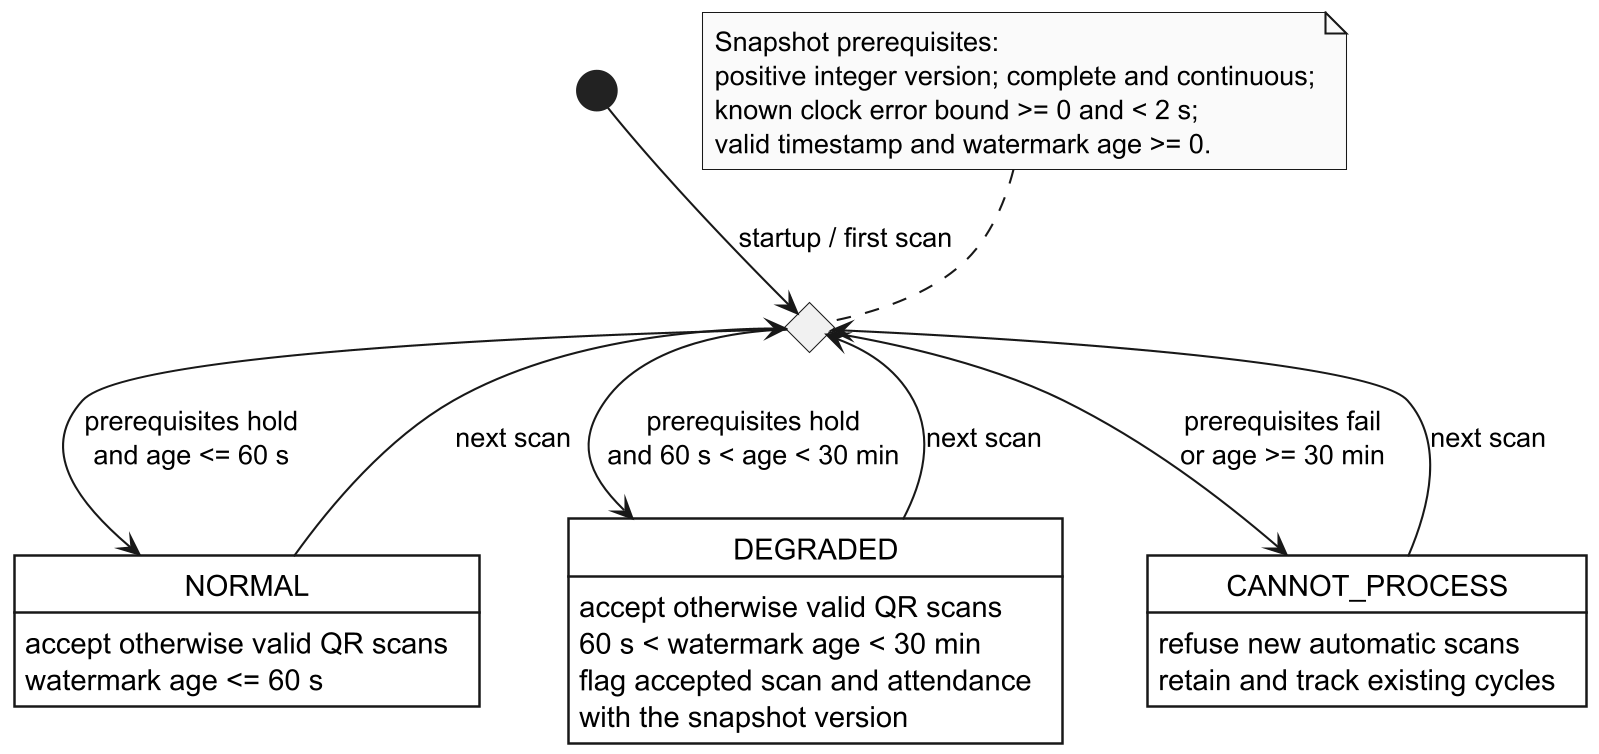
\includegraphics[width=0.9\linewidth]{diagram/deployment/figure-5-3-operating-modes.png}}{\fbox{\parbox{300pt}{\centering\vspace{20pt}Figure being redrawn\vspace{20pt}}}}

\vspace{6pt}
\textbf{Figure 5.3. Operating Modes of a Factory during Connectivity Loss}
\phantomsection\addcontentsline{lof}{figure}{\protect\numberline{5.3}Operating Modes of a Factory during Connectivity Loss}
\end{minipage}

\vspace{10pt}

Figure 5.3 shows the eligibility-mode decision made from the snapshot for every scan, including after restart. NORMAL requires a valid snapshot and a watermark at most 60 seconds old; a valid snapshot older than 60 seconds but younger than 30 minutes gives DEGRADED. Reconnection alone does not select NORMAL: the applied snapshot must meet those conditions. Storage failure is a separate reason to refuse a new opening even when the snapshot mode is NORMAL. CANNOT\_PROCESS does not itself authorize closing; existing cycles still follow the PASSAGE, LANE\_CLEAR, emergency, and durable-write rules. Audit and alerts on entry to and exit from DEGRADED are design requirements. The prototype emits these through in-memory stubs when it enters DEGRADED and returns to NORMAL; it does not emit an end event on transition to CANNOT\_PROCESS. In CANNOT\_PROCESS, guards use the approved manual procedure (Section 5.7.2).

\textbf{How the enhancements mitigate the issue.} Table 5.8 checks each concern from the problem statement against the enhancements and states the risk that remains.

\begin{longtable}{|>{\raggedright\arraybackslash}p{84pt}|>{\raggedright\arraybackslash}p{186pt}|>{\raggedright\arraybackslash}p{141pt}|}
\hline
\multicolumn{1}{|>{\columncolor{tableheader}\centering\arraybackslash}p{84pt}|}{\textbf{Concern}} & \multicolumn{1}{>{\columncolor{tableheader}\centering\arraybackslash}p{186pt}|}{\textbf{Result with E1--E5}} & \multicolumn{1}{>{\columncolor{tableheader}\centering\arraybackslash}p{141pt}|}{\textbf{Remaining risk}} \\
\hline
\endhead
\multicolumn{3}{c}{\rule{0pt}{20pt}\normalsize\phantomsection\addcontentsline{lot}{table}{\protect\numberline{5.8}Mitigation of Connectivity Loss}\textbf{Table 5.8. Mitigation of Connectivity Loss}} \\
\endlastfoot
Lost attendance record & The record and its outbox event are committed at the factory before anything is sent to the central site, and they are delivered later with the same eventId. & The outbox must be large enough for the outage (sized for 48 hours, alerts at 70\% and 85\%, Table 5.5). \\
\hline
Duplicate record & scanId, tokenId, passageEventId, and eventId are each unique, and central consumers use eventId and version to skip events they have already processed. & Missing versions and the outbox backlog have to be monitored (ADR-05). \\
\hline
Gate state unknown & An uncertain opening is queried where the controller supports it and otherwise reconciled, never resent, and the lane stays held until the outcome is known. & A held lane may need a guard to step in during the shift peak. \\
\hline
Out-of-date access rights & Degraded mode lasts less than 30 minutes, and every scan in it is flagged with its snapshot version for Attendance Review. & A revoked employee can still pass during that window, and the flag cannot undo the entry (I-10). \\*
\hline\noalign{\nobreak}
Central site down & Automatic scans stop within about 60 seconds as the shown codes expire, and the manual procedure takes over. & Guard staffing for about 80 arrivals per minute at the peak (Section 5.7.2). \\
\hline
\end{longtable}

\textbf{Example: the opening reply is lost.} Scan S-1 on LANE-BD-01 passes the checks, and ACCEPTED, the token claim, the gate cycle, and the OPEN command are committed in one transaction. The controller may now open the gate, but its reply does not arrive within the time left. Gate Core stores UNDETERMINED and keeps the lane and the token held. If a supported status query returns OPEN\_CONFIRMED, Gate Core records OPENED. Confirmed non-execution produces CONTROLLER\_ERROR. If no query is available or the outcome remains unknown, the scan moves to PENDING\_RECONCILIATION. Gate Core does not resend the OPEN command.

\textbf{What the prototype shows.} The Task 2 code covers E2, E3, and the mode rules of E4 for one factory (Chapter 9). Tests on a real SQLite file show that an UNDETERMINED opening becomes PENDING\_RECONCILIATION without a second openGate, that a controller signal sent twice still gives one attendance record, and that the stored state survives an application restart (\code{test_e2e_sqlite_flows.py}). The NORMAL, DEGRADED, and CANNOT\_PROCESS limits are tested in \code{test_pkg1_snapshot.py}. Site Sync, the broker, and the central site are not built, so delivery after reconnection (E5) is shown only in the design.

\Needspace{9\baselineskip}
\subsubsection*{5.8.2. Exposure of a Static QR Code}

\phantomsection
\addcontentsline{toc}{subsubsection}{5.8.2. Exposure of a Static QR Code}

\textbf{Problem.} A static QR code never changes. Anyone who gets a photo, a screenshot, or a forwarded copy of it can pass the gate and create attendance in the employee's name for as long as the code is accepted, and the system cannot tell the copy from the original. Table 5.9 lists the ways a code can be misused.

\begin{longtable}{|>{\raggedright\arraybackslash}p{40pt}|>{\raggedright\arraybackslash}p{120pt}|>{\raggedright\arraybackslash}p{251pt}|}
\hline
\multicolumn{1}{|>{\columncolor{tableheader}\centering\arraybackslash}p{40pt}|}{\textbf{ID}} & \multicolumn{1}{>{\columncolor{tableheader}\centering\arraybackslash}p{120pt}|}{\textbf{Threat}} & \multicolumn{1}{>{\columncolor{tableheader}\centering\arraybackslash}p{251pt}|}{\textbf{Example}} \\
\hline
\endhead
\multicolumn{3}{c}{\rule{0pt}{20pt}\normalsize\phantomsection\addcontentsline{lot}{table}{\protect\numberline{5.9}Threats from an Exposed QR Code}\textbf{Table 5.9. Threats from an Exposed QR Code}} \\
\endlastfoot
T1 & Copy used later & A colleague keeps a photo of the code and checks in for the employee the next day. \\
\hline
T2 & Copy used at the same time & The same image is shown at two lanes of one factory within a few seconds. \\
\hline
T3 & Copy used at the other factory & A code issued for Binh Duong is shown at Long An. \\
\hline
T4 & Forged or changed code & Someone edits the employee identifier inside the code or builds a new code. \\
\hline
T5 & Leak through a shared channel & A QR image sent by email is forwarded or stays in a mailbox. \\*
\hline\noalign{\nobreak}
T6 & Live sharing & The employee sends a fresh code to a colleague, who scans it before it expires. \\
\hline
\end{longtable}

\textbf{Alternatives considered.} Table 5.10 compares the options we looked at.

\begin{longtable}{|>{\raggedright\arraybackslash}p{110pt}|>{\raggedright\arraybackslash}p{140pt}|>{\raggedright\arraybackslash}p{161pt}|}
\hline
\multicolumn{1}{|>{\columncolor{tableheader}\centering\arraybackslash}p{110pt}|}{\textbf{Option}} & \multicolumn{1}{>{\columncolor{tableheader}\centering\arraybackslash}p{140pt}|}{\textbf{Strength}} & \multicolumn{1}{>{\columncolor{tableheader}\centering\arraybackslash}p{161pt}|}{\textbf{Weakness}} \\
\hline
\endhead
\multicolumn{3}{c}{\rule{0pt}{20pt}\normalsize\phantomsection\addcontentsline{lot}{table}{\protect\numberline{5.10}Alternatives for Protecting the QR Credential}\textbf{Table 5.10. Alternatives for Protecting the QR Credential}} \\
\endlastfoot
Keep the static code and revoke it when a leak is reported & Nothing changes for employees. & A leak is rarely noticed, so revocation comes after the damage. \\
\hline
Static code plus a PIN at the kiosk & Adds a second factor. & Typing a PIN slows the shift-change peak, and a PIN can be shared as easily as the image. \\
\hline
Code that changes on the phone from a shared secret (TOTP style) & Works without a network on the phone. & The secret must be stored on every phone and at every factory, and a leaked secret lets anyone build valid codes. \\
\hline
Short-lived code signed at the central site, bound to one factory and used once (chosen) & The private key stays at the central site, factories need only public keys, and a code is useless after 60 seconds or after its first claim. & The phone needs to reach the central site to get a code, and the code still does not prove who holds the phone. \\
\hline
Code signed by a key kept in the employee's phone & Ties the code to one registered phone. & Needs a device enrollment process and the mobile app on every phone, and does not stop an employee from handing over the phone. \\*
\hline\noalign{\nobreak}
Guard or biometric check of the person at the gate & Checks the person who holds the code. A badge alone would only add another credential that can be lent. & New hardware or extra guard work, slower lanes, and extra personal data to protect (NFR-04). Outside the scope of this design. \\
\hline
\end{longtable}

\textbf{Chosen enhancement.} We use the short-lived signed code of ADR-11 and I-09. QR Credential Issuance at the central site signs a code that holds the token identifier, the employee identifier, the factory, and its validity, and that expires 60 seconds after it is issued. Access Decision at the factory checks the signature with the public key, the validity period, the factory, and the employee's rights in Eligibility Snapshot. Gate Transaction Processor then claims the tokenId in the same transaction as ACCEPTED, so only one scan across all lanes of the factory can use it (Section 7.3). Under assumption I-08, company email only links to the live code screen and never carries a reusable image. Attendance is still created only from a timely PASSAGE linked to a scan that is still OPENED, not from the scan or the opening alone; an emergency-superseded or late passage is retained for review.

\textbf{How the enhancement mitigates the issue.} Table 5.11 maps each threat to the control that stops it and to the risk that is left.

\begin{longtable}{|>{\raggedright\arraybackslash}p{28pt}|>{\raggedright\arraybackslash}p{220pt}|>{\raggedright\arraybackslash}p{163pt}|}
\hline
\multicolumn{1}{|>{\columncolor{tableheader}\centering\arraybackslash}p{28pt}|}{\textbf{ID}} & \multicolumn{1}{>{\columncolor{tableheader}\centering\arraybackslash}p{220pt}|}{\textbf{Control}} & \multicolumn{1}{>{\columncolor{tableheader}\centering\arraybackslash}p{163pt}|}{\textbf{Remaining risk}} \\
\hline
\endhead
\multicolumn{3}{c}{\rule{0pt}{20pt}\normalsize\phantomsection\addcontentsline{lot}{table}{\protect\numberline{5.11}Mitigation of QR Exposure}\textbf{Table 5.11. Mitigation of QR Exposure}} \\
\endlastfoot
T1 & The code expires after 60 seconds, and a claimed tokenId cannot be claimed again, so an old copy is rejected as expired or as a replay. & None after the code has expired or been claimed. \\
\hline
T2 & The claim is part of the ACCEPTED write and is protected by a unique key, so the second scan is rejected and audited. & The first scan wins, and it may be the copy. \\
\hline
T3 & The factory is part of the signed content and is compared with the server's own factory, not with a value sent by the kiosk. & None. \\
\hline
T4 & Any change breaks the signature, and only the central site holds the private key. & Theft of the private key at the central site. \\
\hline
T5 & No reusable image is sent; email only links to the authenticated live display. & I-08 is still an assumption that TMC has to confirm. \\*
\hline\noalign{\nobreak}
T6 & Not blocked. Attendance needs a real passage, and each scan is audited with its lane and time. & A valid, unclaimed copy may win the first scan. If TMC cannot accept this, an independent check of the person at the gate is needed; device binding alone does not prevent sharing a displayed code. \\
\hline
\end{longtable}

\textbf{Example: one image at two lanes.} An employee scans a valid code at LANE-BD-01, and a few seconds later a photo of the same code is shown at LANE-BD-02. The first scan claims the tokenId in the same transaction as ACCEPTED, so the second one is stored as REJECTED with QR\_TOKEN\_REPLAY\_DETECTED and audited with its lane and time. The order could also be the other way round. Whichever accepted scan claims the token first wins. Reuse of that token is rejected, but the stored evidence does not establish who presented it.

\textbf{What the prototype shows.} The Task 2 code verifies the factory side of this enhancement with real Ed25519 keys: signature, expiry, factory binding, and key rotation in \code{test_pkg2_*.py}, two connections claiming one token in \code{test_pkg4_sqlite_repos.py}, and a copied code on another lane rejected with QR\_TOKEN\_REPLAY\_DETECTED in \code{test_e2e_sqlite_flows.py}. The QR issuer in the prototype is only a demo helper, not the central issuing service.

\Needspace{9\baselineskip}
\subsubsection*{5.8.3. Impact on the Architecture}

\phantomsection
\addcontentsline{toc}{subsubsection}{5.8.3. Impact on the Architecture}

Neither enhancement needs a new module or node. They are rules inside modules that already exist, fixed by ADR-02, ADR-05, ADR-06, and ADR-11. Table 5.12 shows where each part lives.

\begin{longtable}{|>{\raggedright\arraybackslash}p{95pt}|>{\raggedright\arraybackslash}p{316pt}|}
\hline
\multicolumn{1}{|>{\columncolor{tableheader}\centering\arraybackslash}p{95pt}|}{\textbf{Module or node}} & \multicolumn{1}{>{\columncolor{tableheader}\centering\arraybackslash}p{316pt}|}{\textbf{Role in the two enhancements}} \\
\hline
\endhead
\multicolumn{2}{c}{\rule{0pt}{20pt}\normalsize\phantomsection\addcontentsline{lot}{table}{\protect\numberline{5.12}Where the Enhancements Live}\textbf{Table 5.12. Where the Enhancements Live}} \\
\endlastfoot
M1 Gate Core (factory) & Access Decision checks the signed code and the operating mode; Gate Transaction Processor stores ACCEPTED and the token claim before openGate, handles uncertain results without resending, and writes attendance with its outbox event. \\
\hline
M2 Turnstile Integration (factory) & Queries the controller about uncertain commands where supported; otherwise Gate Core retains the uncertain outcome for reconciliation. \\
\hline
M4 Access \& Configuration (central) & QR Credential Issuance signs short-lived codes and keeps the private key; the Access Change Feed sends access rights and confirmed watermarks to the factories. \\
\hline
M9 Site Sync (both sites) & Delivers outbox events with their original identifiers and applies access-right updates in the recovery order of Figure 5.2. \\
\hline
M5 Attendance (central) & Attendance Review checks DEGRADED transactions after reconnection and handles reconciliation cases. \\
\hline
M11 Audit, M12 Monitoring & Record rejected replays and the start and end of degraded mode, and raise alerts for degraded mode and outbox capacity. \\
\hline
Factory server and database & Primary and standby with a synchronous copy (Section 5.6.2), so a server failure does not lose the token claims or the outbox. \\*
\hline\noalign{\nobreak}
Central reverse proxy and broker & The proxy runs as an active/standby pair because QR issuing depends on it; the broker has a recovery target that stays below the 30-minute limit (Table 5.5). \\
\hline
\end{longtable}
